% !TEX root = ../main.tex

\section{New mitigations}

By this point, we have discussed 10 solutions to the multiple withdrawal attack and we evaluated them in terms of compatibility with the standard and attack mitigation (recall the summary in Table~\ref{tab:comp}). Since none of them precisely satisfy the constraints of ERC20 standard, we now propose two new solutions to mitigate the attack.

\subsection{Proposal 1: Securing \texttt{approve} method}\label{sec:proposal1}

By implementing CAS \cite{Ref06} in \texttt{approve} method, new allowance can be set atomically after comparing with transferred tokens. This tracking requires adding a new variable to \texttt{transferFrom} method (see Figure~\ref{fig:transfer1}). Since this is an internal variable, it is not visible to already deployed smart contracts and keeps the \texttt{transferFrom} function compatible. Similarly, a block of code is added to the \texttt{approve} function (see Figure~\ref{fig:approve1}) to work in both cases with zero and non-zero allowances. Added code to the \texttt{approve} function, compares new allowance---passed as \texttt{\_tokens} argument to the function---with the current allowance of the spender and already transferred tokens---highlighted as \texttt{allowed[msg.sender][\_spender]} and \texttt{transferred[msg.sender][\_spender]}. Then it decides to increase or decrease current allowance based on this comparison. If the new allowance is less than initial allowance---sum of \texttt{allowance} and \texttt{transferred} variables---it denotes decreasing of allowance, otherwise increasing of allowance was intended. Modified \texttt{approve} function prevents the attack in either increasing or decreasing of the allowance.

Unlike other solutions, there is no need to set allowance from N to 0 and then to M. Token holder can directly change the allowance from N to M which is saving one transaction accordingly. The following examples make functionality of added codes more clear when decreasing or increasing allowance:
 
\begin{figure}[t]
	\centering
	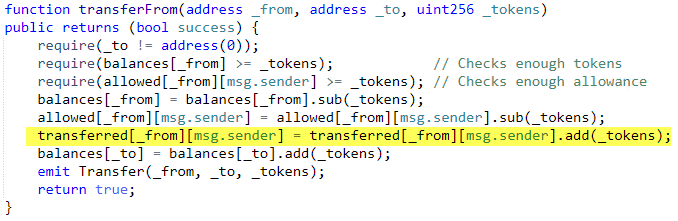
\includegraphics[width=1.0\linewidth]{figures/multiple_withdrawal_14.png}
	\caption{Modified version of \texttt{transferFrom} for keeping track of transferred tokens per spender.\label{fig:transfer1}}
\end{figure}
\begin{comment}
function transferFrom(address _from, address _to, uint256 _tokens) public returns (bool success) {
	require(_to != address(0));
	require(balances[_from] >= _tokens);                 // Checks if approver has enough tokens
	require(allowed[_from][msg.sender] >= _tokens);      // Checks allowance
	balances[_from] = balances[_from].sub(_tokens);
	allowed[_from][msg.sender] = allowed[_from][msg.sender].sub(_tokens);
	transferred[_from][msg.sender] = transferred[_from][msg.sender].add(_tokens);
	balances[_to] = balances[_to].add(_tokens);
	emit Transfer(_from, _to, _tokens);
	return true;
}
\end{comment}

\begin{figure}[t]
	\centering
	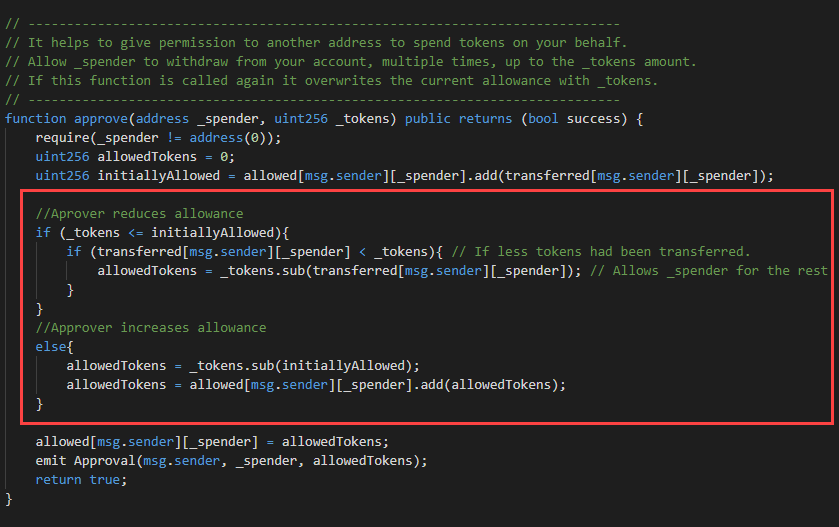
\includegraphics[width=1.0\linewidth]{figures/multiple_withdrawal_15.png}
	\caption{Added code block to \texttt{approve} function to prevent the attack by comparing and setting new allowance atomically.\label{fig:approve1}}
\end{figure}
\begin{comment}
function approve(address _spender, uint256 _tokens) public returns (bool success) {
	require(_spender != address(0));
	uint256 allowedTokens = 0;
	uint256 initiallyAllowed = allowed[msg.sender][_spender].add(transferred[msg.sender][_spender]);
	
	//Aprover reduces allowance
	if (_tokens <= initiallyAllowed){ 
		if (transferred[msg.sender][_spender] < _tokens){ // If less tokens had been transferred.
			allowedTokens = _tokens.sub(transferred[msg.sender][_spender]); // Allows _spender for the rest 
		}
	}
	//Approver increases allowance
	else{ 
		allowedTokens = _tokens.sub(initiallyAllowed);
		allowedTokens = allowed[msg.sender][_spender].add(allowedTokens);
	}
	
	allowed[msg.sender][_spender] = allowedTokens;
	emit Approval(msg.sender, _spender, allowedTokens);
	return true;
}
\end{comment}
\subsubsection*{Scenario A} Alice approves Bob for spending 100 tokens and then decides to decrease it to 10 tokens.
\begin{enumerate}
	\item Alice approves Bob for transferring 100 tokens.
	\item After a while, Alice decides to reduce Bob’s allowance from 100 to 10 tokens.
	\item Bob noticed Alice’s new transaction and transfers 100 tokens by front-running.
	\item Bob’s allowance is 0 and \texttt{transferred} is 100 (set by \texttt{transferFrom} function).
	\item Alice’s transaction is mined and checks initial allowance (100) with new allowance (10).
	\item As it is reducing, \texttt{transferred} tokens (100) is compared with new allowance (10). Since Bob already transferred more tokens, his allowance will be set to 0.
	\item Bob is not able to move more than initial 100 approved tokens.
\end{enumerate}

\subsubsection*{Scenario B} Alice approves Bob for spending 100 tokens and then decides to increase it to 120 tokens.
\begin{enumerate}
	\item Alice approves Bob for transferring 100 tokens.
	\item After a while, Alice decides to increase Bob’s allowance from 100 to 120 tokens.
	\item Bob noticed Alice’s new transaction and transfers 100 tokens by front-running.
	\item Bob’s allowance is 0 and \texttt{transferred} is 100.
	\item Alice’s transaction is mined and checks initial allowance (100) with new allowance (120).
	\item As it is increasing, new allowance (120) will be subtracted from transferred tokens (100).
	\item 20 tokens will be added to Bob’s allowance.
	\item Bob would be able to transfer more 20 tokens (120 in total as Alice wanted).\newline
\end{enumerate}

In order to evaluate functionality of the new \texttt{approve} and \texttt{transferFrom} functions, we have implemented a standard ERC20 token (TKNv1\footnote{https://rinkeby.etherscan.io/address/0x8825bac68a3f6939c296a40f c8078d18c2f66ac7}) along side the proposed ERC20 token (TKNv2\footnote{https://rinkeby.etherscan.io/address/0xf2b34125223ee54dff48f715 67d4b2a4a0c9858b}) on Rinkeby test network. Result of tests for different input values shows that TKNv2 can address multiple withdrawal attack by making front-running gain ineffective. Moreover, we compared these two tokens in term of gas consumption. TokenV2.\texttt{approve} function uses almost the same amount of gas as TokenV1.\texttt{approve}, however, gas consumption of TokenV2.\texttt{transferFrom} is around 47\% more than TokenV1.\texttt{transferFrom} (see Figure~\ref{fig:gas}). This difference is because of maintaining a new mapping variable for tracking transferred tokens. In term of compatibility, working with standard wallets (\eg MetaMask) have not raised any transfer issue. This shows compatibility of the token with existing wallets.

\begin{figure}[t]
	\centering
	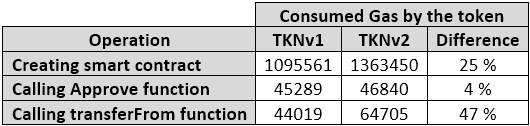
\includegraphics[width=1.0\linewidth]{figures/multiple_withdrawal_22.png}
	\caption{Comparison of gas consumption between standard implementation of ERC20 token (TKNv1) and secured implementation of it (TKNv2).\label{fig:gas}}
\end{figure}
\begin{comment}
function transferFrom(address _from, address _to, uint256 _tokens) public returns (bool success) {
	require(_to != address(0));
	require(balances[_from] >= _tokens);                // Checks if approver has enough tokens
	require(_tokens <= (
		(allowed[_from][msg.sender] > transferred[_from][msg.sender]) ? 
		allowed[_from][msg.sender].sub(transferred[_from][msg.sender]) : 0)
		);                              // Prevents token transfer more than allowance
	
	balances[_from] = balances[_from].sub(_tokens);
	transferred[_from][msg.sender] = transferred[_from][msg.sender].add(_tokens);
	balances[_to] = balances[_to].add(_tokens);
	emit Transfer(_from, _to, _tokens);
	return true;
}
\end{comment}
In summary, we could use CAS pattern to implement a secure \texttt{approve} method that can mitigate the attack effectively. However, it violates one of ERC20 specifications that says "If this function is called again it overwrites the current allowance with \texttt{\_value}". This implementation of \texttt{approve} method adjusts allowance based on transferred tokens. Essentially, it would not be possible to secure the \texttt{approve} method without adjusting the allowance. Considering the below scenario:

\begin{enumerate}
	\item Alice decides to change Bob's allowance from N to M (M less than N in this example).
	\item Bob transfers N tokens by front running and \texttt{transferred} variable sets to N.
	\item Alice's transaction is mined and \texttt{approve} method detects token transfer. If \texttt{approve} method does not adjust the allowance based on transferred tokens, it has to set it to M---to conform with the standard---which is allowing Bob to transfer more M tokens.
\end{enumerate}
Therefore, \texttt{approve} method has to adjust the allowance according to transferred tokens, not based on passed input values to the \texttt{approve} method. Overall, there is no solution to secure \texttt{approve} method while adhering specification of ERC20 standard.

\subsection{Proposal 2: Securing \texttt{transferFrom} method}\label{sec:proposal2}

As an alternative solution to Proposal 1, we can think of securing \texttt{transferFrom} method instead of \texttt{approve} function. As specified by ERC20 standard (see figure~\ref{fig:standard}), the goal here is to prevent spender from transferring more tokens than allowed. Based on this assumption, we should not consider allowance as the main prevention factor. Transferred tokens can be considered as the main variable in our calculations. For example in the below situation, we can prevent the attack by securing \texttt{transferFrom} method and keeping \texttt{approve} function untouched to set allowance as specified by the token holder:
\begin{enumerate}
	\item Alice allowed Bob for transferring 100 tokens and decides to set it to 70 after a while.
	\item Bob front runs Alice’s transaction and transfers 100 tokes (legitimate transfer).
	\item Alice transaction is mined and sets Bob allowance to 70 by the default \texttt{approve} method.
	\item Bob noticed new allowance and tries to move new tokens by running \texttt{transferFrom(\_Bob,70)}. Since he already transferred more than 70, his transaction fails and prevents multiple withdrawal. Additionally, Bob’s allowance stays as 70, although transferred tokens shows 100.
\end{enumerate}
Here, \texttt{allowance} value can be considered as maximum allowance. It indicates that Bob is eligible to transfer up to specified limit if he has not already transferred any tokens. This impression is completely in accordance with ERC20 standard (see figure~\ref{fig:standard}). In fact, there is no relation between allowance (\texttt{allowed[\_from][msg.sender]}) and transferred tokens (\texttt{transferred[\_from][msg.sender]}). The first variable shows maximum transferable tokens by a spender and can be changed irrelative to transferred tokens (\ie \texttt{approve} method does not check transferred tokens). If Bob has not already transferred that much of tokens, he would be able to transfer difference of it---\texttt{allowed[\_from][msg.sender].sub(transfer red[\_from][msg.sender]}). In other words, \texttt{transferred} variable is a life time variable that accumulates transferred tokens regardless of allowance changes. This token is implemented as TKNv3\footnote{https://rinkeby.etherscan.io/address/0x5d148c948c01e1a61e280c8 b2ac39fd49ee6d9c6} on Rinkby network and passed compatibility checks by transferring tokens between standard wallets. In terms of gas consumption, \texttt{transferFrom} function needs at about 37\% more gas than standard \texttt{transferFrom} implementation which is acceptable for having a secure ERC20 token.

\begin{figure}[t]
	\centering
	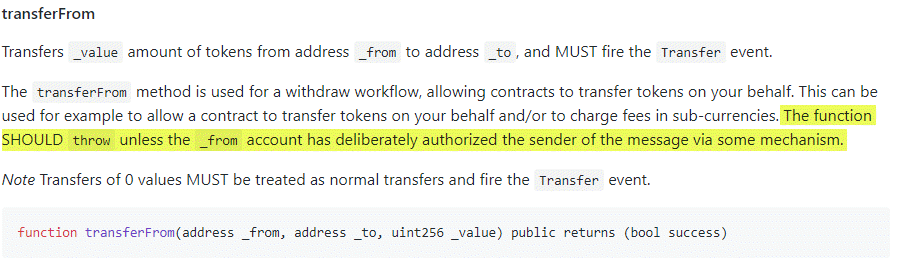
\includegraphics[width=1.0\linewidth]{figures/multiple_withdrawal_30.png}
	\caption{ERC20 \texttt{transferFrom} method definition that emphasizes on throwing an exception when the spender is not authorized to move tokens.\label{fig:standard}}
\end{figure}

\begin{figure}[t]
	\centering
	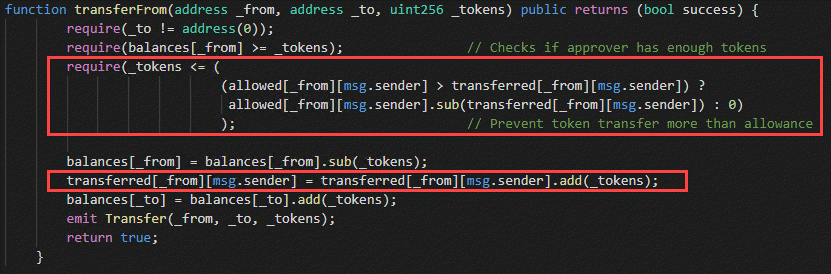
\includegraphics[width=1.0\linewidth]{figures/multiple_withdrawal_31.png}
	\caption{Securing \texttt{transferFrom} method instead of \texttt{approve} method can mitigate the attack by preventing more token transfer than allowed.\label{fig:transfer2}}
\end{figure}